\subsection{Introduction to Functions}
To talk about functions, is to talk about relationships. Take the `<' sign, this is a relationship.
$x < y$ means $x$ relates to $y$, such that $x$ is less than $y$.\\

\noindent
\centering
Let $a=\{1,2,3,4\}$, $b=\{0,1,2,3\}$. Let $R$ be the relation `<', $aRb$ yields:

\vspace{1em}
\begin{figure}[ht]
    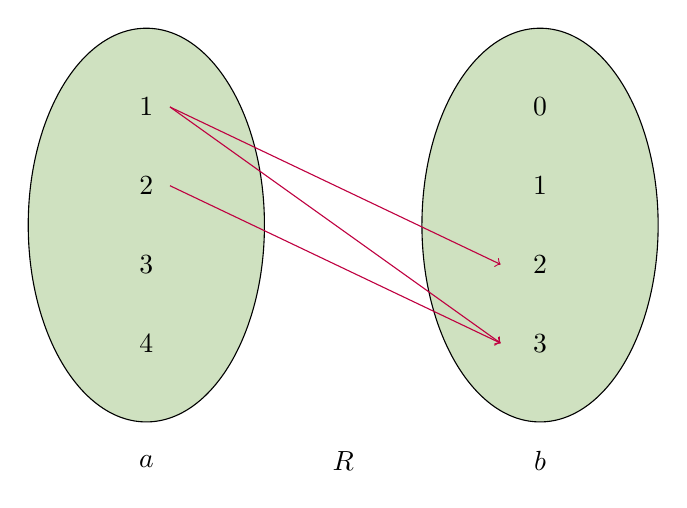
\begin{tikzpicture}
        % Draw the sets
        \draw[black, fill=OliveGreen!20] (-3,0) ellipse (1.5 and 2.5);
        \draw[black, fill=OliveGreen!20] (2,0) ellipse (1.5 and 2.5);


        % Labels for the elements in the first set
        \node at (-3,1.5) {1};
        \node at (-3,.5) {2};
        \node at (-3,-.5) {3};
        \node at (-3,-1.5) {4};
        \node at (-3,-3) {$a$};

        % Labels for the elements in the second set
        \node at (2,1.5) {0};
        \node at (2,.5) {1};
        \node at (2,-.5) {2};
        \node at (2,-1.5) {3};
        \node at (2,-3) {$b$};

        \node at (-.5,-3) {$R$};

        % Draw the arrow
        %1
        \draw[->, purple] (-2.7,1.5) -- (1.5,-.5);
        \draw[->, purple] (-2.7,1.5) -- (1.5,-1.5);

        %2
        \draw[->, purple] (-2.7,.5) -- (1.5,-1.5);
    \end{tikzpicture}
    \caption{\centering $R={(1,2),(1,3)(2,3)}
    \label{fig:relates}
\end{figure}


